\subsection{平行四边形及其性质}\label{subsec:czjh1-4-3}

两组对边分别平行的四边形叫做\zhongdian{平行四边形}。
如图 \ref{fig:czjh1-4-8} 四边形 $ABCD$  中, $AB \pingxing DC$, $AD \pingxing BC$,
那么四边形 $ABCD$ 是平行四边形。
平行四边形用符号 “$\pxsbx$” 表示, 平行四边形 $ABCD$ 记作 “$\pxsbx ABCD$”,
读作 “平行四边形 $ABCD$”。

\begin{figure}[htbp]
    \centering
    \begin{minipage}[b]{7cm}
        \centering
        \begin{tikzpicture}
    \tkzDefPoints{0/0/B,  2.5/0/C, 3.3/1.5/D, 0.8/1.5/A}
    \tkzDrawPolygon(A,B,C,D)
    \tkzLabelPoints[left](A,B)
    \tkzLabelPoints[right](C,D)
\end{tikzpicture}


        \caption{}\label{fig:czjh1-4-8}
    \end{minipage}
    \qquad
    \begin{minipage}[b]{7cm}
        \centering
        \begin{tikzpicture}
    \tkzDefPoints{0/0/B,  2.5/0/C, 3.3/1.5/D, 0.8/1.5/A}
    \tkzDrawPolygon(A,B,C,D)
    \tkzDrawSegment[dashed](A,C)
    \extkzLabelAngel[0.3](B,A,C){$1$}
    \extkzLabelAngel[0.5](A,C,B){$2$}
    \extkzLabelAngel[0.3](D,C,A){$3$}
    \extkzLabelAngel[0.5](C,A,D){$4$}
    \tkzLabelPoints[left](A,B)
    \tkzLabelPoints[right](C,D)
\end{tikzpicture}


        \caption{}\label{fig:czjh1-4-9}
    \end{minipage}
\end{figure}

下面研究平行四边形的一些性质。
我们已经学过了三角形,如果画出平行四边形的一条对角线,
就把平行四边形分成两个三角形,可以利用三角形的性质来研究平行四边形。

首先研究平行四边形的两组对边、两组对角的关系。

作 $\pxsbx ABCD$ 的对角线 $AC$, 将它分成 $\triangle ABC$ 和 $\triangle CDA$(图 \ref{fig:czjh1-4-9})。

$\because$ \quad $AB \pingxing CD$, $AD \pingxing BC$,

$\therefore$ \quad $\angle 1 = \angle 3$, $\angle 2 = \angle 4$。

又 $\because$ \quad $AC = CA$,

$\therefore$ \quad $\triangle ABC \quandeng \triangle CDA$。

$\therefore$ \quad $AB = CD$, $CB = AD$, $\angle B = \angle D$。

又 $\because$ \quad $\angle 1 + \angle 4 = \angle 2 + \angle 3$,

$\therefore$ \quad $\angle A = \angle C$。

由此得到:

\begin{dingli}[平行四边形性质定理1]
    平行四边形的对角相等。
\end{dingli}

\begin{dingli}[平行四边形性质定理2]
    平行四边形的对边相等。
\end{dingli}

如图 \ref{fig:czjh1-4-10}, $L_1 \pingxing l_2$, $AB$、 $CD$ 是 $l_1$、$l_2$ 之间的任意两条平行线段,
显然, $ABDC$ 是平行四边形。 因为平行四边形的对边相等, 所以 $AB = CD$。 由此得到:

\begin{tuilun}[推论]
    夹在两条平行线间的平行线段相等。
\end{tuilun}

\begin{figure}[htbp]
    \centering
    \begin{minipage}[b]{7cm}
        \centering
        \begin{tikzpicture}
    \tkzDefPoints{0/0/B,  2.5/0/D, 3.3/1.5/C, 0.8/1.5/A}
    \tkzDrawLines[add=0.3 and 0.3](A,C  B,D)
    \tkzDrawSegments(A,B  C,D)
    \tkzLabelSegment[pos=0, left=.8cm](A,C){$l_1$}
    \tkzLabelSegment[pos=0, left=.8cm](B,D){$l_2$}
    \tkzLabelPoints[above](A,C)
    \tkzLabelPoints[below](B,D)
\end{tikzpicture}


        \caption{}\label{fig:czjh1-4-10}
    \end{minipage}
    \qquad
    \begin{minipage}[b]{7cm}
        \centering
        \begin{tikzpicture}
    \tkzDefPoints{0/0/B, -2/0/b1, 2/0/b2, 0/1.5/A, -2/1.5/a1, 2/1.5/a2}
    \tkzDrawSegments(a1,a2  b1,b2  A,B)
    \tkzMarkRightAngle(A,B,b2)
    \tkzLabelSegment[pos=0, left](a1,a2){$l_1$}
    \tkzLabelSegment[pos=0, left](b1,b2){$l_2$}
    \tkzLabelPoints[above](A)
    \tkzLabelPoints[below](B)
\end{tikzpicture}


        \caption{}\label{fig:czjh1-4-11}
    \end{minipage}
\end{figure}


从推论可以知道,如果两条直线平行,那么一条直线上所有各点,到另一条直线的距离都相等。
两条平行线中,一条直线上任意一点到另一条直线的距离,叫做\zhongdian{这两条平行线的距离}。
如图 \ref{fig:czjh1-4-11}, $l_1 \pingxing l_2$,  $A$ 是 $l_1$ 上的任意一点, $AB \perp l_2$,
$B$ 是垂足, 线段 $AB$ 的长就是 $l_1$、 $l_2$ 的距离。

平行四边形还有下面性质:

\begin{dingli}[平行四边形性质定理3]
    平行四边形的对角线互相平分。
\end{dingli}

\begin{wrapfigure}[7]{r}{5cm}
    \centering
    \begin{tikzpicture}
    \tkzDefPoints{0/0/B,  2.5/0/C, 3.3/1.5/D, 0.8/1.5/A}
    \tkzInterLL(A,C)(B,D)  \tkzGetPoint{O}
    \tkzDrawPolygon(A,B,C,D)
    \tkzDrawSegments(A,C  B,D)
    \extkzLabelAngel[0.3](B,A,C){$1$}
    \extkzLabelAngel[0.4](D,B,A){$2$}
    \extkzLabelAngel[0.4](B,D,C){$3$}
    \extkzLabelAngel[0.3](D,C,A){$4$}
    \tkzLabelPoints[left](A,B)
    \tkzLabelPoints[right](C,D)
    \tkzLabelPoints[above](O)
\end{tikzpicture}


    \caption{}\label{fig:czjh1-4-12}
\end{wrapfigure}


已知: $\pxsbx ABCD$, 对角线 $AC$、$BD$ 相交于点 $O$ (图\ref{fig:czjh1-4-12})。

求证: $OA = OC$, $OB = OD$。

\zhengming $\because$ \quad 在 $\pxsbx ABCD$ 中, $AB \pingxing CD$,

$\therefore$ \quad $\angle 1 = \angle 4$, $\angle 2 = \angle 3$。

又 $\because$ \quad $AB = CD$ (平行四边形的对边相等),

$\therefore$ \quad $\triangle OAB \quandeng \triangle OCD$。

$\therefore$ \quad $OA = OC$, $OB = OD$。

我们知道, 三角形具有稳定性,而四边形就没有稳定性。
可以利用四边形的不稳定性制成活动的平行四边形框(图 \ref{fig:czjh1-4-13}),
汽车的防护链(图 \ref{fig:czjh1-4-14})等。

\begin{figure}[htbp]
    \centering
    \begin{minipage}[b]{8cm}
        \centering
        \includegraphics[width=7cm]{../pic/czjh1-ch4-13.png}
        \caption{}\label{fig:czjh1-4-13}
    \end{minipage}
    \qquad
    \begin{minipage}[b]{6cm}
        \centering
        \includegraphics[width=3cm]{../pic/czjh1-ch4-14.png}
        \caption{}\label{fig:czjh1-4-14}
    \end{minipage}
\end{figure}



\begin{wrapfigure}[8]{r}{6cm}
    \centering
    \begin{tikzpicture}
    \tkzDefPoints{0/0/B,  2.0/0/C, 1.2/1.5/A}
    \tkzDefLine[parallel=through A](B,C)  \tkzGetPoint{a}
    \tkzDefLine[parallel=through B](A,C)  \tkzGetPoint{b}
    \tkzDefLine[parallel=through C](A,B)  \tkzGetPoint{c}
    \tkzInterLL(A,a)(B,b)  \tkzGetPoint{C'}
    \tkzInterLL(A,a)(C,c)  \tkzGetPoint{B'}
    \tkzInterLL(B,b)(C,c)  \tkzGetPoint{A'}
    \tkzDefLine[altitude](B,A,C)  \tkzGetPoint{D}
    \tkzDefLine[altitude](A,B,C)  \tkzGetPoint{E}
    \tkzDefLine[altitude](A,C,B)  \tkzGetPoint{F}

    \tkzDrawPolygon(A,B,C)
    \tkzDrawPolygon(A',B',C')
    \tkzDrawSegments(A,D  B,E  C,F)
    \tkzMarkRightAngle[size=0.2](A,D,C)
    \tkzMarkRightAngle[size=0.2](B,E,C)
    \tkzMarkRightAngle[size=0.2](C,F,B)

    \tkzLabelPoints[above](A)
    \tkzLabelPoints[below](A', D)
    \tkzLabelPoints[left](C',B)
    \tkzLabelPoints[right](C,B')
    \tkzLabelPoints[above right=-0.3em](E)
    \tkzLabelPoints[above left=-0.3em](F)
\end{tikzpicture}


    \caption{}\label{fig:czjh1-4-15}
\end{wrapfigure}

\liti 过 $\triangle ABC$ 的顶点 $A$、$B$、$C$,分别引对边的平行线,
它们两两相交于 $A'$、$B'$、$C'$。求证:$\triangle ABC$ 的三条高是
$\triangle A'B'C'$ 三边的垂直平分线。

已知:如图 \ref{fig:czjh1-4-15}, $C'B' \pingxing BC$, $C'A' \pingxing AC$, $B'A' \pingxing AB$;
$AD \perp BC$, $BE \perp CA$, $CF \perp AB$。

求证:$AD$、$BE$、$CF$ 分别是 $C'B'$、$C'A'$、$A'B'$ 的垂直平分线。

\zhengming $\because$ \quad $C'B' \pingxing BC$, $C'A' \pingxing AC$, $B'A' \pingxing AB$,

$\therefore$ \quad $BC = C'A$ (夹在两条平行线间的平行线段相等)。

同理 \quad $BC = AB'$

$\therefore$ \quad $C'A = AB'$。

又 $\because$ \quad $AD \perp BC$,

$\therefore$ \quad $AD \perp C'B'$。

所以. $AD$ 是 $C'B'$ 的垂直平分线。

同理 \quad $BE$、$CF$ 分别是 $C'A'$、$A'B'$ 的垂直平分线。


在前一章里,我们已经证明过三角形三边的垂直平分线交于一点,
由于例 1 中的 $\triangle A'B'C'$ 三边的垂直平分线就是 $\triangle ABC$ 的三条高。
可见,三角形的三条高也相交于一点。


\begin{wrapfigure}[8]{r}{5cm}
    \centering
    \begin{tikzpicture}
    \tkzDefPoints{0/0/B,  2.5/0/C, 3.3/1.5/D, 0.8/1.5/A}
    \tkzInterLL(A,C)(B,D)  \tkzGetPoint{O}
    \tkzDefMidPoint(O,A)  \tkzGetPoint{M}
    \tkzDefMidPoint(O,C)  \tkzGetPoint{N}
    \tkzDrawPolygon(A,B,C,D)
    \tkzDrawSegments(A,C  B,D  B,M  D,N)
    \tkzLabelPoints[left](A,B)
    \tkzLabelPoints[right](C,D)
    \tkzLabelPoints[above right=-0.4em](M)
    \tkzLabelPoints[below left=-0.4em](N)
    \tkzLabelPoints[above](O)
\end{tikzpicture}


    \caption{}\label{fig:czjh1-4-16}
\end{wrapfigure}

\liti 已知:$\pxsbx ABCD$ 中, 对角线 $AC$ 和 $BD$ 相交于点 $O$,
$M$、$N$ 分别是 $OA$、$OC$ 的中点(图 \ref{fig:czjh1-4-16})。

求证:$BM = DN$, $BM \pingxing DN$。

\zhengming $\because$ \quad 四边形 $ABCD$ 是平行四边形,

$\therefore$ \quad $OB = OD$, $OA = OC$ (平行四边形的对角线互相平分)。

\begin{enhancedline}
$\because$ \quad $OM = \exdfrac{1}{2} OA$, $ON = \exdfrac{1}{2} OC$,

$\therefore$ \quad $OM = ON$。
\end{enhancedline}

又 $\because$ \quad $\angle MOB = \angle NOD$,

$\therefore$ \quad $\triangle MOB \quandeng \triangle NOD$。

$\therefore$ \quad $BM = DN$, $\angle BMO = \angle DNO$。

$\therefore$ \quad $BM \pingxing DN$。


\begin{lianxi}

\xiaoti{举出日常生活中常见的平行四边形的一些例子。}

\xiaoti{已知: 在 $\pxsbx ABCD$ 中, $AE \perp BC$, $CF \perp AD$, $E$、$F$ 是垂足。\\
    求证: $\triangle ABE \quandeng \triangle CDF$。
}

\xiaoti{如图 \ref{fig:czjh1-4-12}, 已知 $O$ 是 $\pxsbx ABCD$ 的对角线交点, 如果 $AC = 24\;\haomi$,
    $BD = 38\;\haomi$, $AD = 28\;\haomi$, 求 $\triangle OBC$ 的周长。
}

\end{lianxi}

